\subsection{Real Morse events in the singular category}

Let $\tau\in\R$ and consider the two functions
\begin{equation}
 a^+_\tau(x,y)=x^2+y^2-\tau,
 \qquad
 a^-_\tau(x,y)=x^2-y^2-\tau.
 \label{eq:morse-assignments}
\end{equation}
Their common critical set in each slice is the origin.  On
$\R^2\setminus\{0\}$ define
\begin{equation}
 g^\pm_\tau=
 \frac{4(x^2+y^2)}
 {\mu^2+\lambda^2(a^\pm_\tau)^2}
 (\dd x^2+\dd y^2).
 \label{eq:morse-aeg-metric}
\end{equation}

\begin{proposition}[AEG Morse bifurcations]
\label{prop:aeg-morse-bifurcations}
For every $\tau$, the tuple
\[
 (\R^2,\{0\},g^\pm_\tau,a^\pm_\tau;\mu,\lambda)
\]
is a singular AES.  Its total zero incidence in $\R^2\times\R_\tau$ is smooth,
but projection to $\tau$ has a critical point at $(0,0,0)$.

For $a^+_\tau$, the zero changes from empty to a singular point and then to a
circle as $\tau$ crosses zero.  For $a^-_\tau$, the two hyperbolic branches
reconnect through the four regular rays meeting at the singular origin when
$\tau=0$.
\end{proposition}

\begin{proof}
The Euclidean norm squared of $\dd a^\pm_\tau$ is $4(x^2+y^2)$, so
Corollary~\ref{cor:singular-realization} gives the AEG equation and local
essentiality.  Define
$A^\pm(x,y,\tau)=a^\pm_\tau(x,y)$.  Since
$\partial_\tau A^\pm=-1$, zero is a regular value of the total function; hence
$(A^\pm)^{-1}(0)$ is smooth.  The parameter projection restricted to it is
critical precisely when the spatial derivative vanishes, which happens at the
origin.  The stated zero sets follow directly from
$x^2+y^2=\tau$ and $x^2-y^2=\tau$.
\end{proof}

\begin{figure}[ht]
\centering
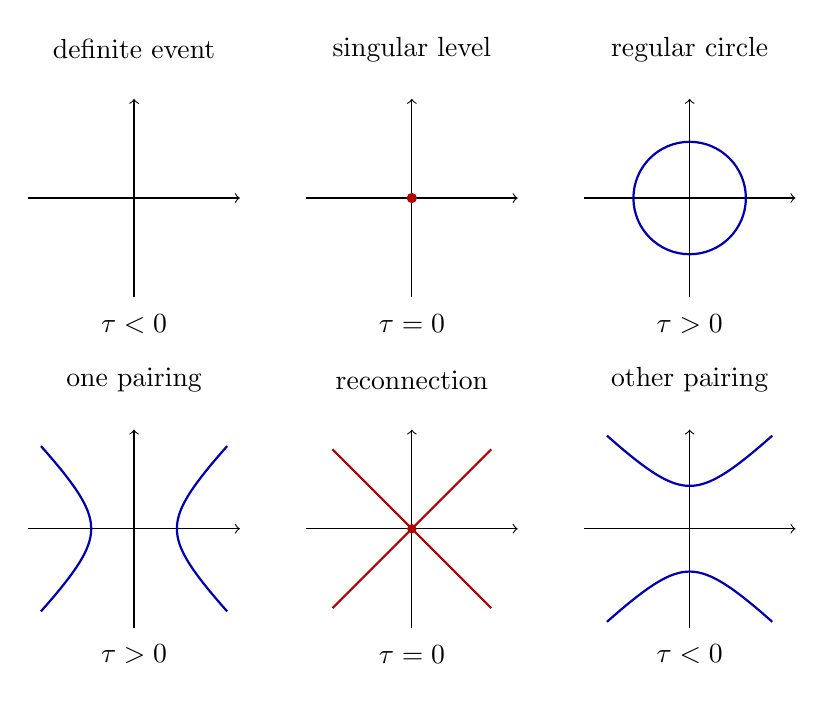
\begin{tikzpicture}[scale=0.84]
  \begin{scope}[xshift=0cm]
    \node at (0,2.25) {definite event};
    \draw[->] (-1.6,0)--(1.6,0);
    \draw[->] (0,-1.5)--(0,1.5);
    \node at (0,-1.9) {$\tau<0$};
  \end{scope}
  \begin{scope}[xshift=4.2cm]
    \node at (0,2.25) {singular level};
    \draw[->] (-1.6,0)--(1.6,0);
    \draw[->] (0,-1.5)--(0,1.5);
    \fill[red!70!black] (0,0) circle (2.2pt);
    \node at (0,-1.9) {$\tau=0$};
  \end{scope}
  \begin{scope}[xshift=8.4cm]
    \node at (0,2.25) {regular circle};
    \draw[->] (-1.6,0)--(1.6,0);
    \draw[->] (0,-1.5)--(0,1.5);
    \draw[blue!70!black,thick] (0,0) circle (0.85);
    \node at (0,-1.9) {$\tau>0$};
  \end{scope}
  \begin{scope}[yshift=-5.0cm]
    \node at (0,2.25) {one pairing};
    \draw[->] (-1.6,0)--(1.6,0);
    \draw[->] (0,-1.5)--(0,1.5);
    \draw[blue!70!black,thick,domain=-1.25:1.25,samples=80]
      plot ({sqrt(0.42+\x*\x)},\x);
    \draw[blue!70!black,thick,domain=-1.25:1.25,samples=80]
      plot ({-sqrt(0.42+\x*\x)},\x);
    \node at (0,-1.9) {$\tau>0$};
  \end{scope}
  \begin{scope}[xshift=4.2cm,yshift=-5.0cm]
    \node at (0,2.25) {reconnection};
    \draw[->] (-1.6,0)--(1.6,0);
    \draw[->] (0,-1.5)--(0,1.5);
    \draw[red!70!black,thick] (-1.2,-1.2)--(1.2,1.2);
    \draw[red!70!black,thick] (-1.2,1.2)--(1.2,-1.2);
    \fill[red!70!black] (0,0) circle (2pt);
    \node at (0,-1.9) {$\tau=0$};
  \end{scope}
  \begin{scope}[xshift=8.4cm,yshift=-5.0cm]
    \node at (0,2.25) {other pairing};
    \draw[->] (-1.6,0)--(1.6,0);
    \draw[->] (0,-1.5)--(0,1.5);
    \draw[blue!70!black,thick,domain=-1.25:1.25,samples=80]
      plot (\x,{sqrt(0.42+\x*\x)});
    \draw[blue!70!black,thick,domain=-1.25:1.25,samples=80]
      plot (\x,{-sqrt(0.42+\x*\x)});
    \node at (0,-1.9) {$\tau<0$};
  \end{scope}
\end{tikzpicture}
\caption{Real AEG-compatible Morse examples.  The red point is a declared
essential singularity.  The pictures record zero topology only; they are not a
classification of metric germs.}
\label{fig:real-morse-events}
\end{figure}

The proposition exhibits the key phenomenon
\[
 \text{smooth total zero incidence}
 \not\!\Longrightarrow
 \text{zero tube}.
\]
At the event, it is the projection that fails to be a submersion.

\subsection{A regular-to-singular fold wall}

A related family makes all noncritical slices regular rather than retaining a
singular point away from the zero.  Put
\[
 A(x,y,\tau)=e^x(y^2-\tau).
\]
For $\tau\ne0$, the spatial derivative never vanishes; for $\tau=0$, it vanishes
along the entire line $y=0$.  On the regular locus use
\begin{equation}
 g_\tau=
 \frac{e^{2x}\bigl((y^2-\tau)^2+4y^2\bigr)}
 {\mu^2+\lambda^2e^{2x}(y^2-\tau)^2}
 (\dd x^2+\dd y^2).
 \label{eq:fold-wall-metric}
\end{equation}
For $\tau<0$ the zero fiber is empty, for $\tau>0$ it consists of two parallel
lines, and for $\tau=0$ it is the singular line $y=0$.  The metric degenerates
there and the line is locally essential.  This is a verified wall-crossing family,
but it is nonproper and its singular stratum is one-dimensional.

\subsection{The complex branch model}

Real scalar zeros and complex roots have different local models.  Let
$(w,\tau)\in\C^2$ and consider
\begin{equation}
 F(w,\tau)=w^2-\tau.
 \label{eq:complex-branch-model}
\end{equation}
The incidence $F^{-1}(0)$ is a smooth complex curve parameterized by
$w\mapsto(w,w^2)$.  Its projection to the $\tau$-plane is a two-sheeted branched
cover with a single simple branch point at the origin.

On the boundary circle $\tau=\varepsilon e^{i\theta}$, the two roots are
\begin{equation}
 w_\pm(\theta)=\pm\sqrt\varepsilon\,e^{i\theta/2}.
 \label{eq:half-twist-roots}
\end{equation}
They remain distinct for every boundary parameter and exchange after one circuit.
The boundary therefore carries the standard half-twist in $B_2$; the collision is
at the center of the filling, not on the boundary braid.

\begin{proposition}[Simple polynomial discriminant normal form]
\label{prop:simple-discriminant-normal-form}
Let a holomorphic family of monic polynomials, parameterized by a complex
$d$-manifold, meet the polynomial discriminant transversely at a parameter where
exactly one root has multiplicity two and all other roots are simple.  After
holomorphic changes of root and parameter coordinates
$\tau=(\tau_1,\ldots,\tau_d)$, its local root incidence is the disjoint union of
simple graphs and one copy of
\[
 w^2=\tau_1,
\]
with $\tau_2,\ldots,\tau_d$ as spectator coordinates.
\end{proposition}

\begin{proof}
Separate the simple roots by the holomorphic implicit-function theorem.  The
remaining quadratic factor has the form $w^2+b(\tau)w+c(\tau)$.  Translating
$w$ removes the linear term.  Its discriminant is a holomorphic function of the
parameter; transversality makes that function the first member $\tau_1$ of a
local coordinate system.  Rescaling $\tau_1$ gives
\eqref{eq:complex-branch-model}, while the remaining parameter coordinates pass
through unchanged.
\end{proof}

Restricting $\tau$ to the real axis gives two real roots for $\tau>0$ and two
imaginary roots for $\tau<0$.  Their four half-arcs meet at the branch point.  This
four-valent picture is a real slice of a complex branched cover, not a regular
four-valent zero of a real assignment.

\subsection{Smooth and holomorphic fillings}

Section~\ref{sec:braids} realizes every braid by a family that is smooth in the
loop parameter and holomorphic in the spatial coordinate $w$.  Extending such a
family over a parameter disc while remaining holomorphic in both variables is a
stronger demand.  Algebraic-function boundaries are constrained by
quasipositivity \cite{Rudolph1983AlgebraicFunctions}.  Thus the statements
\begin{align*}
 &\text{every braid has an arithmetic-holomorphic spatial realization},\\
 &\text{every braid bounds a holomorphic AEG root filling}
\end{align*}
are not equivalent; the first is proved below, while the second is false without
restrictions.

\begin{problem}[AEG-natural singular fillings]
\label{prob:natural-fillings}
Determine which branch signs and global braided surfaces arise when the parameter
dependence is constrained by expression history or by a natural connection, rather
than chosen as an arbitrary smooth or holomorphic polynomial family.
\end{problem}
